\chapter{Extracción de características}\label{cha:extraccion_caracteristicas}

\AddToShipoutPictureBG*{\put(0,0){%
        \parbox[b][\paperheight]{\paperwidth}{%
            \vfill
            \centering
            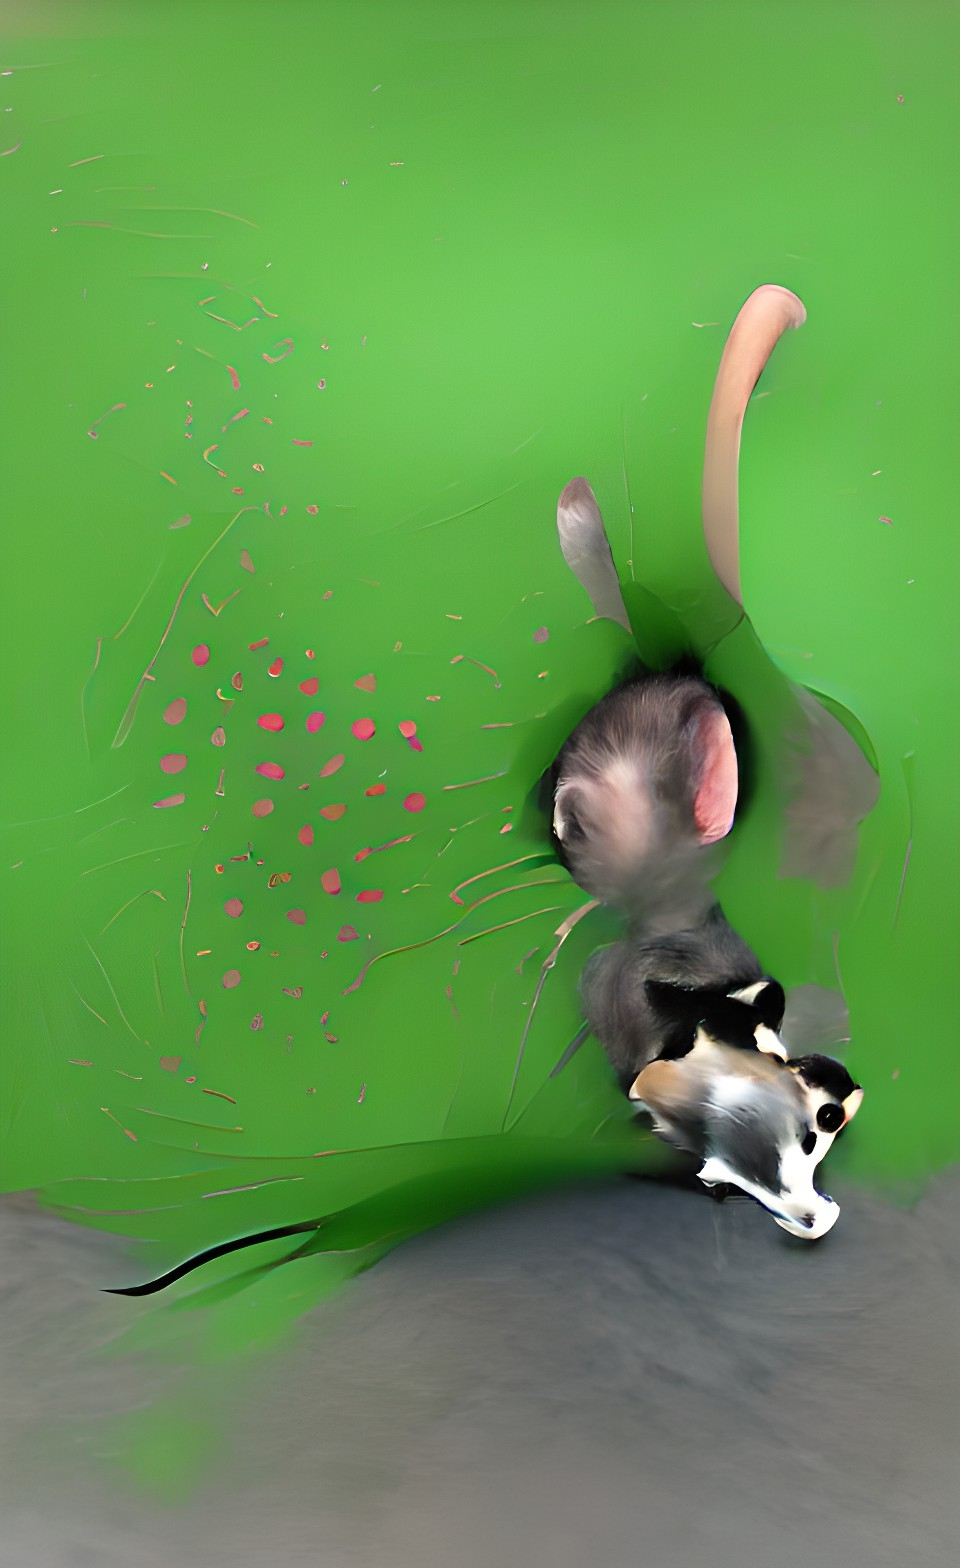
\includegraphics[width=\paperwidth,height=\paperheight,keepaspectratio]{%
                figuras/caratulas/extraccion_de_caracteristicas.jpg}\vfill
        }}}

\AddToShipoutPicture*{
    \begin{tikzpicture}[overlay, remember picture]
        \fill[white, opacity=0.75] (20, 24) rectangle (1, 21);
    \end{tikzpicture}}

\clearpage

El comportamiento animal es inherentemente dinámico y evoluciona en el tiempo. Para capturar la estructura temporal del comportamiento es necesario medir variables biofísicas de los animales a lo largo del tiempo. Estas son diversas características que están asociadas a las partes del cuerpo, las poses y la dinámica de los movimientos de los animales estudiados. El objetivo último del proceso de extracción de características es encontrar conjuntos de variables adecuados que mejor describan los tipos de comportamientos que queremos estudiar (esto es, que mejor separen en categorías a los patrones de movimiento o a los estados biofísicos de los animales). Debido a su fácil incorporación en los experimentos comportamentales, en este trabajo consideramos únicamente características que se extraen de los registros de video de los ratones, durante la ejecución de la tarea rotarod. Sin embargo, existen otros tipos de señales biofísicas que se utilizan para describir el comportamiento, como por ejemplo los registros de audio de vocalizaciones de aves y otros animales, como ratones, murciélagos, ballenas o primates \cite{miranda_mouse_vocals, sainburg_birdsong_umap}.

\section{Captura de movimiento}\label{sec:captura_movimiento}

Recientemente, una de las aplicaciones de aprendizaje automático que más impactó en la neurociencia del comportamiento es la captura de movimiento sin marcadores \cite{datta_computational_neuroethology}. Los avances en captura de movimiento permiten medir las posiciones de las partes del cuerpo de los animales, y de otros puntos de interés, sin la necesidad de colocar marcadores físicos adicionales ni de utilizar cámaras especializadas.

En este trabajo, utilizamos DeepLabCut, una herramienta de código abierto para estimar las posiciones de marcadores digitales definidos por el usuario (\autoref{fig:capitulo2_posiciones}) \cite{mathis_deeplabcut}. DeepLabCut utiliza redes neuronales artificiales profundas, que se entrenan con pocos fotogramas de video (típicamente, entre 50 y 200 fotogramas) para adecuarlas a las condiciones experimentales particulares del experimento, alcanzado una precisión equivalente a la humana. Con esta herramienta, se procesaron más de 10 millones de fotogramas (más de 30 hs de video), provenientes de las filmaciones de 2 cámaras (frontal y trasera) que registraron un total de 250 pruebas rotarod, realizadas por 10 ratones. Cada ratón realizó 5 pruebas por día, durante 5 días de entrenamiento, siendo la duración promedio ($\pm$ desviación estándar) de una prueba ($220 \pm 50$) s, lo cual equivale a 22\,000 fotogramas a una frecuencia de muestreo de 100 Hz.

\begin{figure}[htbp]
    \centering
    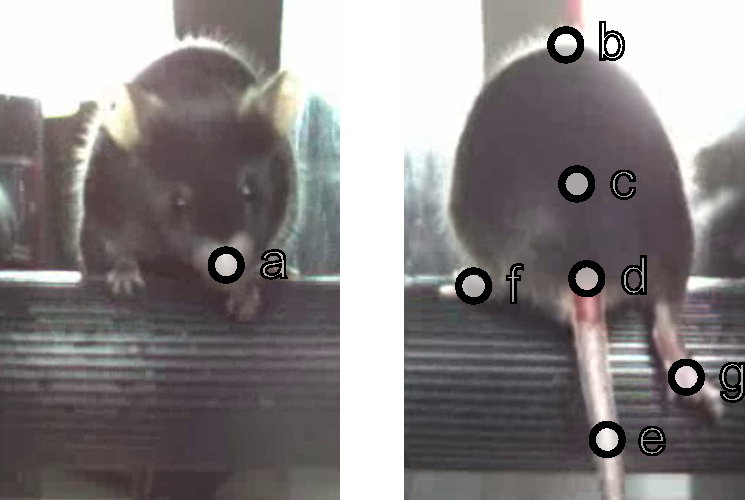
\includegraphics[width=0.65\linewidth]{figuras/capitulo2/captura_movimiento.pdf}
    \caption{\textbf{Captura de movimiento.} Marcadores digitales utilizados en el seguimiento de las partes del cuerpo del ratón.
        (Izquierda) Cámara frontal. (Derecha) Cámara trasera.
        Marcadores: (a) nariz, (b) espalda, (c) centro de masa, (d) base de la cola, (e) mitad de la cola, (f) pata trasera izquierda, (g) pata trasera derecha.}
    \label{fig:capitulo2_captura_movimiento}
\end{figure}

Si bien la tecnología de captura de movimiento avanzó mucho con la introducción de las redes neuronales artificiales, las posiciones estimadas por DeepLabCut deben procesarse \textit{a posteriori} para corregir problemas en la captura de movimiento. Se aplicaron, en el siguiente orden, un filtro de mediana, una transformación de perspectiva, un filtro de Kalman, un filtro de \textit{clipping} y un filtro de \textit{trimmed mean} sobre las señales. Aprovechamos que la captura de movimiento con DeepLabCut devuelve las \textit{likelihoods} de las estimaciones de las posiciones de los marcadores y utilizamos esas \textit{likelihoods} para calcular los errores en el filtro de Kalman. La implementación en Python de estos filtros se puede encontrar en el repositorio \href{https://github.com/alvaro-concha/animal-behavior-preprocessing}{\color{blue}{animal-behavior-preprocessing}} y los parámetros utilizados se pueden consultar en el archivo de configuración \href{https://github.com/alvaro-concha/animal-behavior-preprocessing/blob/main/animal_behavior_preprocessing/config.py}{\color{blue}{\texttt{config.py}}}. Desafortunadamente, este procesamiento de las señales reduce su frecuencia de muestreo efectiva alrededor de 30 Hz. El motivo del procesamiento es corregir las posiciones de los marcadores digitales cuando se producen oclusiones totales o parciales de los mismos, reducir el \textit{switching} entre marcadores similares (por ejemplo, confusión entre los marcadores de las patas izquierda y derecha) y compatibilizar los registros de las cámaras frontal y trasera con la transformación de perspectiva, para llevar las posiciones medidas al mismo sistema de referencia.

Una vez llevadas al mismo sistema de referencia usando la transformación de perspectiva, se combinaron las capturas de movimiento de ambas cámaras. La transformación de perspectiva se computó para cada filmación tomando como referencia a las 4 esquinas visibles del cilindro rotarod en el compartimento donde se ubica el ratón. Estas 4 esquinas se llevaron a un sistema de referencia en el que forman un rectángulo de 5.7 cm de ancho por 3 cm de alto, de acuerdo a las dimensiones del aparato rotarod. Así, se obtuvieron las posiciones en el tiempo de varios marcadores, cada uno descritos por una posición horizontal y vertical (\autoref{fig:capitulo2_posiciones}). La posición de la nariz del ratón se obtuvo usando la cámara frontal y las posiciones de la espalda, centro de masa, base de la cola, mitad de la cola y patas traseras usando la cámara trasera (\autoref{fig:capitulo2_captura_movimiento}).

\clearpage

\section{Ángulos entre partes del cuerpo}\label{sec:angulos_entre_partes}

Una vez procesadas y combinadas las posiciones de los marcadores de ambas cámaras, estas se utilizan para calcular los ángulos sostenidos entre diferentes partes del cuerpo del ratón. Los ángulos entre marcadores son invariantes ante traslaciones y rotaciones rígidas y cambios de escala. Por lo tanto, trabajar con ángulos permite ignorar diferencias de tamaño entre individuos, aunque puede perderse información relacionada con la posición y la orientación del ratón y sus partes del cuerpo sobre el cilindro. Para el cálculo de los ángulos es necesario definir tripletes (i j k) con i, j, k símbolos de los marcadores, con el que se calcula el ángulo entre los vectores $\vec{\mathrm{ij}}$ y $\vec{\mathrm{jk}}$. Al conectar los tripletes con líneas se obtienen esqueletos que representan los ángulos extraídos (\autoref{fig:capitulo2_angulos_esqueleto}). Estos ángulos adoptan rangos de valores diferentes (\autoref{fig:capitulo2_angulos}), por lo que es necesario estandarizarlos para que todos tengan el mismo rango de valores. El motivo de esta estandarización es volver comparables a los ángulos que varían poco con los que varían mucho, y que estos últimos no dominen en la representación comportamental a causa de la mayor escala de su rango de valores.

\begin{figure}[htbp]
    \centering
    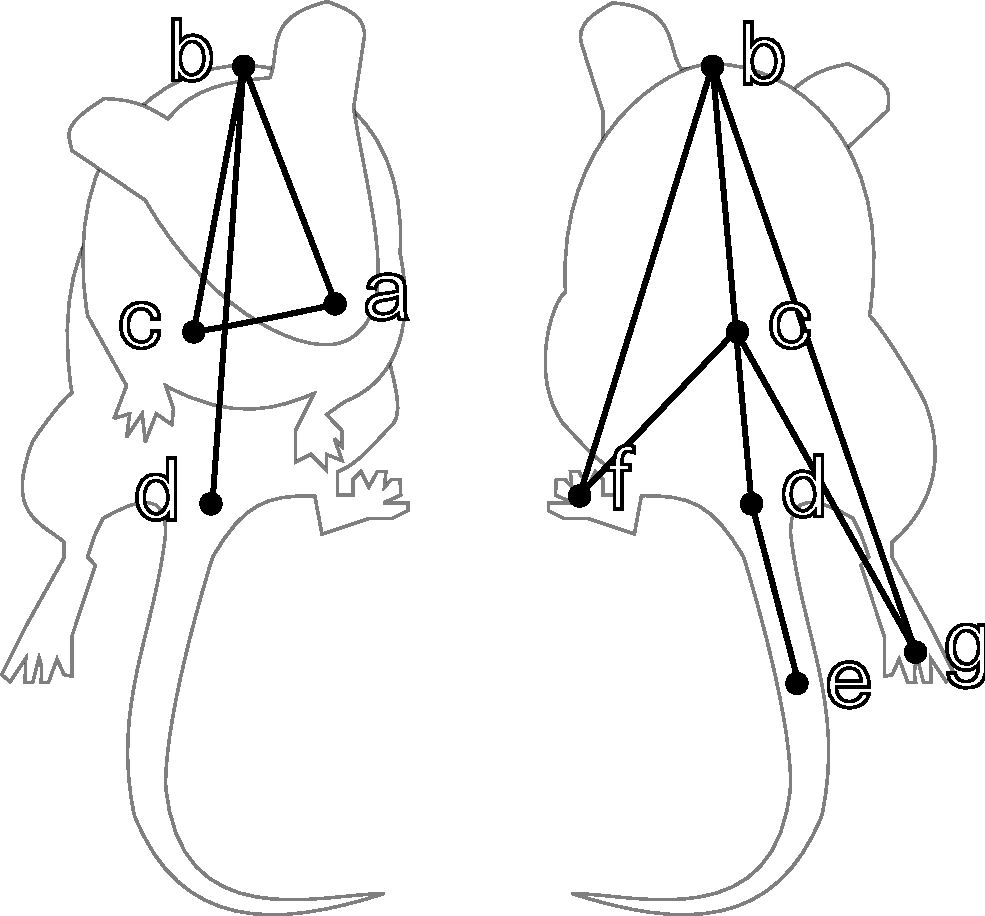
\includegraphics[width=0.5\linewidth]{figuras/capitulo2/angulos_esqueleto.pdf}
    \caption{\textbf{Ángulos de partes del cuerpo.} Esqueletos (líneas y polígonos) sobre ilustraciones de la silueta del ratón, con los que se calcularon los ángulos entre marcadores.
        (Izquierda) Frente (Derecha) Dorso.
        Marcadores: (a) nariz, (b) espalda, (c) centro de masa, (d) base de la cola, (e) mitad de la cola, (f) pata trasera izquierda, (g) pata trasera derecha.}
    \label{fig:capitulo2_angulos_esqueleto}
\end{figure}

\section{Espectros \textit{wavelet} de los ángulos}\label{sec:espectros_wavelet}

Para capturar la dinámica del movimiento de los ratones a diferentes escalas temporales simultáneamente se realiza una transformada \textit{wavelet} sobre los ángulos de las partes del cuerpo del ratón en función del tiempo. La transformada \textit{wavelet} en una convolución entre una señal (en nuestro caso, los ángulos de partes del cuerpo) y una función que depende del tiempo (el \textit{wavelet} propiamente dicho) que depende de un parámetro de escala temporal.  Al variar este parámetro de escala se exploran componentes de diferentes frecuencias presentes en la señal de interés. En particular, para tener mayor sensibilidad a la ocurrencia de intervalos de movimiento periódico, utilizamos \textit{wavelets} de tipo Morlet \cite{berman_mapping}. De esta manera, se obtuvieron las componentes de potencia espectral de las señales en 50 canales de frecuencia, distribuidos diádicamente (esto es, uniformemente en escala logarítmica) desde 0.1 Hz hasta 10 Hz (\autoref{fig:capitulo2_espectros_wavelet}). Estas componentes espectrales varían en el tiempo, al igual que las señales originales, con una resolución temporal de 10 ms. En total, al finalizar el cálculo de cada espectro \textit{wavelet}, se obtienen 50 nuevas variables por cada ángulo. Por lo tanto, pasamos de 10 ángulos entre partes del cuerpo a 500 variables que describen sus componentes espectrales. De esta manera, podemos capturar combinaciones de movimientos de diferentes partes del cuerpo del animal a distintas frecuencias.

Los espectros \textit{wavelet} son invariantes ante pequeñas traslaciones temporales (cambios de fase) en la señal, por lo que se pierde información respecto de las fases de las señales y las diferencias de fase entre las mismas. Esto significa que los espectros \textit{wavelet} pueden ignorar información sobre la sincronización entre partes del cuerpo, si es que esta información se manifiesta por medio de una diferencia de fase en el movimiento de los ángulos (\autoref{fig:capitulo4_mi_mean_wav_scaler_stp} y \autoref{fig:capitulo4_mi_pca_wav_scaler_stp}). A su vez, los espectros \textit{wavelet} de los ángulos entre partes del cuerpo heredan algunas de sus propiedades, y son también invariantes ante traslaciones y rotaciones rígidas de los marcadores y cambios de escala espaciales. Que la transformada \textit{wavelet} sea invariante ante tantas operaciones matemáticas puede parecer una desventaja, pero en ciertas situaciones es en realidad una virtud. Al ser tan robustos frente a varios tipos de perturbaciones, los espectros \textit{wavelet} de los ángulos de partes del cuerpo de animales permiten generalizar fácilmente a diferentes condiciones experimentales, e incluso, permiten que se puedan analizar diferentes especies de animales con la misma técnica, concentrándose solamente en los aspectos que tienen en común la dinámica de sus movimientos.

\section{Características de pasos}\label{sec:caracteristicas_pasos}

Una manera alternativa de extraer características comportamentales es diseñando nuestra propia ingeniería de características. Esto significa aplicar nuestro conocimiento del dominio del comportamiento animal para definir las características que nos interesen particularmente. Una ventaja de este enfoque es que podemos calcular características que sean directamente interpretables y que en pocas variables capturen información relevante del sistema. Como contrapartida, una ingeniería de características muy específica puede consumir mucho tiempo de desarrollo y puede ser difícil de generalizar a otros conjuntos de datos o dominios de problemas.

En este trabajo, definimos un conjunto de características asociadas a los pasos ejecutados por los ratones (\autoref{fig:capitulo2_caracteristicas_de_pasos}). Para ello, aprovechamos que las posiciones verticales de las patas traseras presentan máximos y mínimos locales cada vez que el ratón realiza un paso. Por lo tanto, podemos calcular derivadas de estas señales y determinar de manera relativamente sencilla los tiempos en los que el ratón da un paso. Conociendo estos instantes de tiempo, se obtienen las alturas mínima y máxima de las patas traseras en el entorno del tiempo del paso; la amplitud del paso como la diferencia entre estas alturas máxima y mínima; la velocidad del paso como el máximo local en la primera derivada de la posición vertical de la pata trasera; el desfasaje entre los pasos de ambas patas; y la frecuencia con la que el ratón da pasos con cada pata.

Una vez que tenemos calculados los eventos de ocurrencia de pasos y sus características asociadas, hacemos estadística sobre ellos. Para capturar la manera en que los eventos de pasos evolucionan en el tiempo, calculamos su promedio y desviación estándar en una ventana móvil. Esta ventana abarca 11 pasos consecutivos: lo suficientemente grande como para hacer estadística robusta, pero lo suficientemente pequeña como para capturar variaciones en la estrategia comportamental del ratón en escalas de tiempo de entre 1 s a 10 s (\autoref{fig:capitulo2_estadistica_de_pasos}).

\begin{figure}[htbp]
    \centering
    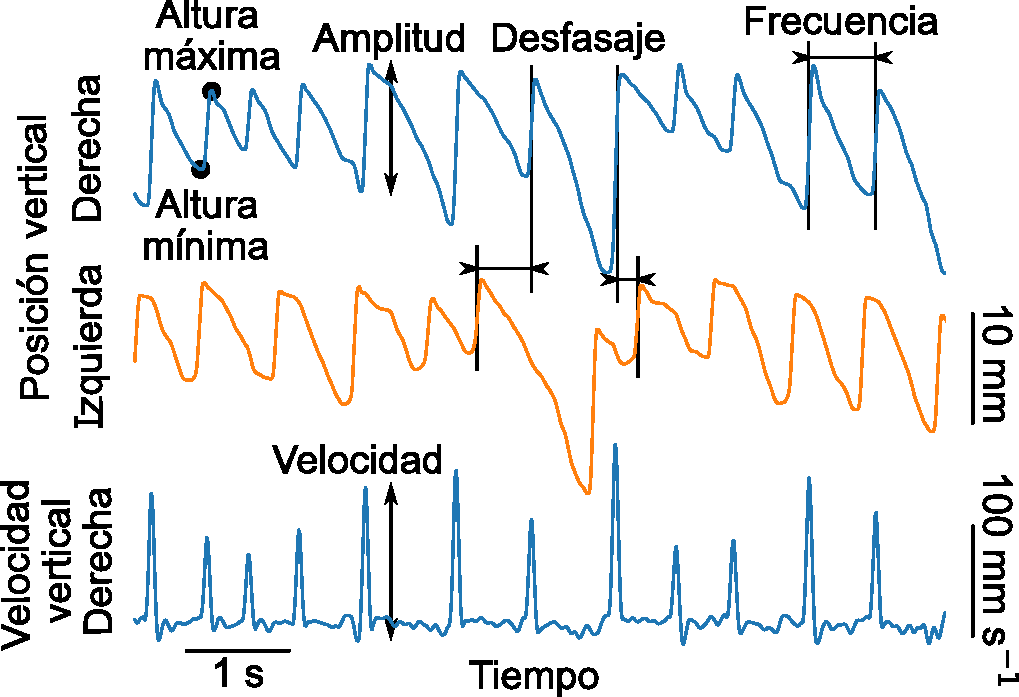
\includegraphics[width=0.65\linewidth]{figuras/capitulo2/caracteristicas_de_pasos.pdf}
    \caption{\textbf{Medición de las características de pasos.}
        Ilustración de las diferentes características asociadas a los pasos de las patas traseras.
        Este ejemplo se centra en la pata derecha.}
    \label{fig:capitulo2_caracteristicas_de_pasos}
\end{figure}

\begin{figure}[htbp]
    \centering
    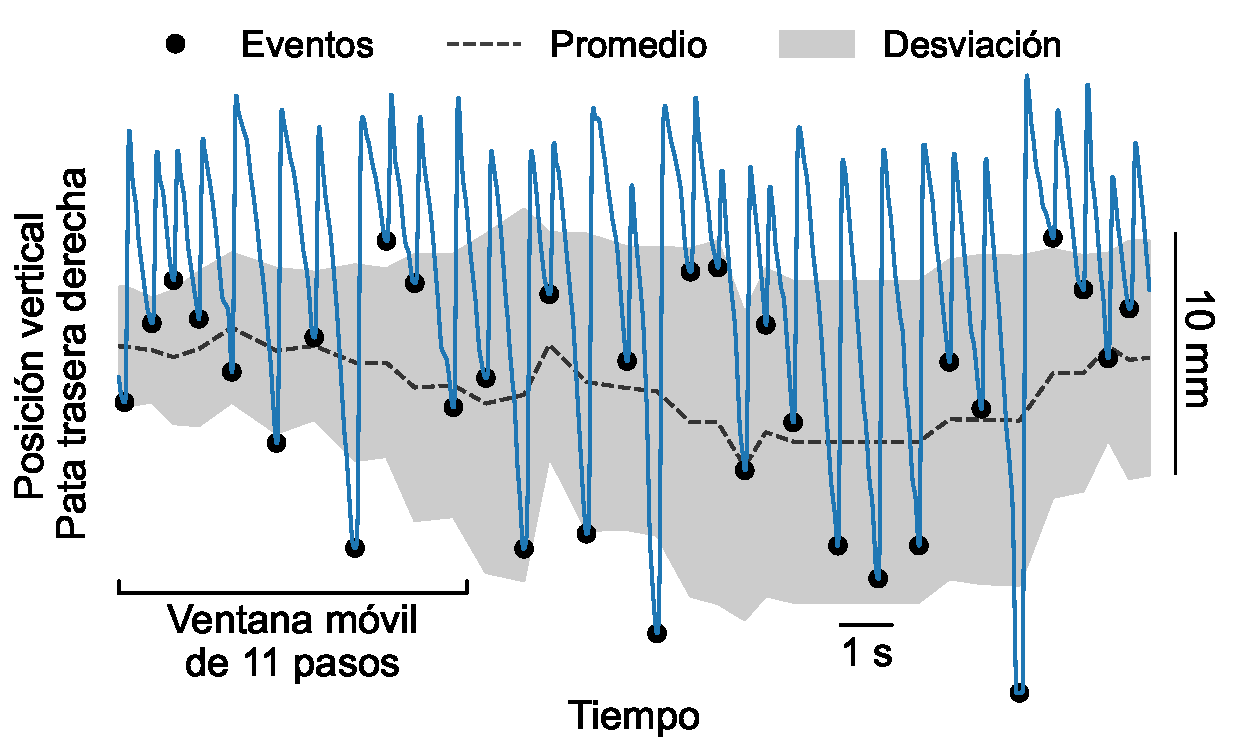
\includegraphics[width=0.8\linewidth]{figuras/capitulo2/estadistica_de_pasos.pdf}
    \caption{\textbf{Estadísticas de las características de pasos.}
        Estimación del promedio y de la desviación estándar de las características de los pasos de las patas traseras.
        Las estadísticas se calculan usando ventanas móviles de 11 pasos consecutivos, sobre las patas izquierda y derecha por separado.
        Este ejemplo se centra en la altura mínima de la pata derecha como característica.}
    \label{fig:capitulo2_estadistica_de_pasos}
\end{figure}